%=======================================================================
% Label-Free Compositional DGA Representations and a Surveillance-Bias
% Caution for Transformer Risk Screening
% Thibaut Faucheux — CESI / KMUTNB — Research Initiation, 2026
%
% Build:  pdflatex main && bibtex main && pdflatex main && pdflatex main
% (or use latexmk -pdf main.tex). Requires the IEEEtran class.
%=======================================================================
\documentclass[conference]{IEEEtran}
\IEEEoverridecommandlockouts

\usepackage{cite}
\usepackage{amsmath,amssymb,amsfonts}
\usepackage{graphicx}
\usepackage{booktabs}
\usepackage{xcolor}
\usepackage{url}
\graphicspath{{../results/figures/}}

% Inline TODO marker — grep for "TODO" before submission.
\newcommand{\todo}[1]{\textcolor{red}{[TODO: #1]}}

\begin{document}

\title{Label-Free Compositional DGA Representations and a
Surveillance-Bias Caution for Transformer Risk Screening}

\author{\IEEEauthorblockN{Thibaut Faucheux}
\IEEEauthorblockA{CESI Engineering School, France \\
KMUTNB, Bangkok, Thailand \\
Email: thibautfaucheux1@gmail.com}
\and
\IEEEauthorblockN{Dr. Rattanakorn Phadungthin}
\IEEEauthorblockA{College of Industrial Technology \\
KMUTNB, Bangkok, Thailand}}

\maketitle

\begin{abstract}
Dissolved Gas Analysis (DGA) interpretation for power transformers remains
rule-based (IEC ratios, Rogers, the Duval Triangle), expert-dependent, and
label-scarce. This paper makes three contributions, learned \emph{without any fault
labels}, on a longitudinal field dataset of 4563 samples from 628 transformers
(2019--2024). First, we show that representing each sample by the centred log-ratio (CLR) of its
combustible-gas composition separates fault \emph{type} from gassing \emph{severity}
by construction: clustering a two-dimensional \emph{linear} projection of the CLR
recovers Duval fault-type structure (adjusted Rand index $0.55$ vs $0.16$ for raw
concentrations), while a neural autoencoder (SD-CAE) and an adversarial
disentanglement term add nothing over this linear pipeline---negative results we
report. Second, and importantly, we show that the field-event notes commonly used to
validate such models are \emph{confounded by surveillance bias}: a trivial
sampling-count predicts logged events as well as the gas chemistry does, and a
label-free risk score loses its apparent forward validity once this is controlled---a caution
for the DGA machine-learning literature, for which we give a confound-free
chemistry-based evaluation. Third, we build a label-free health/risk screening index
(severity, acetylene-aware, temporal, and anomaly terms) that outranks conventional
severity baselines, reported together with the confound floor. Our results indicate that
label-free compositional representations are a useful basis for DGA fault-type discovery, and
that---at least in this fleet---a trivial sample count can dominate operator-logged event labels,
so DGA risk models validated on such labels should report a sample-count confound floor.
\end{abstract}

\begin{IEEEkeywords}
label-free representation learning, dissolved gas analysis, compositional data analysis,
fault diagnosis, label bias, transformer condition monitoring
\end{IEEEkeywords}

\section{Introduction}
% DRAFT (2026-06-17). Prose to own/refine; see docs/problem_statement.md. Keep claims modest.

Power transformers are among the most critical and expensive assets in an electrical
network, and an in-service failure can cause extended outages and high repair costs.
Dissolved Gas Analysis (DGA) is the most widely used technique for the early detection
of incipient faults: thermal and electrical stresses decompose the insulating oil and
paper, releasing characteristic gases---hydrogen, methane, ethane, ethylene, acetylene,
and the carbon oxides---whose relative amounts indicate the type of fault
\cite{ieee_c57104,duval2002review}.

Conventional interpretation methods, namely the IEC~60599 ratios, the Rogers ratios, and
the Duval Triangle, are rule-based. They encode expert knowledge as fixed thresholds,
require an expert to apply and arbitrate, and return a ``not determined'' result for a
non-negligible share of samples \cite{iec60599,duval2002review}. Supervised machine
learning can reach very high accuracy; a recent example fuses the conventional methods
into a single score and feeds an ensemble classifier, reporting $99.17\%$ accuracy
\cite{hybrid_aiscore2026}. Such methods, however, require labelled fault data---and often
the conventional rules themselves as inputs---which utilities rarely have at fleet scale.

This paper studies a label-free alternative on a real operational dataset of 4{,}563 main-tank
samples from 628 transformers (2019--2024), and makes three contributions. We first observe
that representations built on gas concentrations encode overall gassing \emph{magnitude} rather
than fault \emph{type}, and show that the centred log-ratio (CLR) of the combustible-gas
composition separates the two by construction, raising agreement with the Duval fault types
from an adjusted Rand index of $0.16$ to $0.55$ with a simple linear projection; a neural
autoencoder (SD-CAE) and an adversarial disentanglement term add nothing, which we report as
negative ablations. We then show, second, that the
field-event notes routinely used to validate such models are, in this fleet, \emph{confounded by
surveillance bias}: a trivial sample count out-predicts the gas chemistry, and a label-free score
built from each unit's early history loses its apparent forward validity once this count is
controlled---a caution we support with a confound-free,
chemistry-defined evaluation. Third, we build a label-free health/risk screening index that
outranks conventional severity baselines, reported together with this confound floor.

The contributions of this work are:
\begin{itemize}
  \item a label-free \emph{severity-disentangled compositional representation}: the centred
        log-ratio of the combustible-gas composition, on which a linear two-dimensional
        projection recovers Duval fault-type structure (ARI $0.16\rightarrow0.55$); the neural
        (SD-CAE) and adversarial-independence variants are reported as negative ablations;
  \item a finding that, in this fleet, the field-event label used to validate such models is
        confounded by surveillance bias---a trivial sample count out-predicts the gas chemistry
        and the apparent forward validity
        vanishes once it is controlled---together with a confound-free, chemistry-defined
        evaluation target;
  \item a label-free health/risk screening index (severity, acetylene-aware, temporal, and
        anomaly terms) that outranks conventional severity baselines, reported against the
        confound floor.
\end{itemize}

The remainder of the paper is organised as follows. Section~\ref{sec:related} reviews related
work; Section~\ref{sec:data} describes the dataset and preprocessing; Section~\ref{sec:method} the
method; and Sections~\ref{sec:exp}--\ref{sec:results} the experiments and results, before the
conclusion.

\section{Related Work}
\label{sec:related}

We organise prior work along the trajectory mapped by a recent 34-page survey
\cite{ramarao2026review}: rule-based interpretation, supervised machine learning, and
unsupervised / representation learning. We then add the point that motivates this paper:
how such models are \emph{validated}.

\textbf{Conventional DGA interpretation.}
The dominant methods are rule-based: the key-gas method, the IEC~60599 and Rogers gas
ratios, and the Duval Triangle and Pentagon
\cite{iec60599,ieee_c57104,duval2002review,duval2008ltc,duval2001interp}. They are simple and
interpretable but rely on fixed thresholds, require expert judgement, and leave borderline
cases ``not determined''. The current IEEE guide bases its gas-level norms on the 90th and
95th percentiles of a large population and embeds the Duval Triangle as an interpretation
aid \cite{ieee_c57104}.

\textbf{Supervised machine learning for DGA.}
Most learning-based work casts fault diagnosis as supervised classification, using neural
networks \cite{zhang1996ann}, support vector machines \cite{bacha2012svm,fei2009svmga}, and
more recently ensembles and deep models; the survey reports accuracies rising from
$\sim$85--95\% (classical ML, few hundred samples) to $>$97\% (deep learning, $\geq$5000
samples) at the cost of opacity and data hunger \cite{ramarao2026review}. A representative
recent system fuses the four conventional methods into a single ``AI-score'' feature and
reaches $99.17\%$ \cite{hybrid_aiscore2026}, but it requires fault labels \emph{and} the
conventional rules as inputs. The recent transformer \emph{Health Index} literature is
likewise supervised: it predicts an expert-defined health score, so it needs that score as a
label. The survey names prognostics and remaining-useful-life estimation as the open frontier.

\textbf{Unsupervised and representation learning.}
Autoencoders \cite{hinton2006reducing} and variational autoencoders \cite{kingma2014vae}
learn compact representations without labels, and statistical-ML reviews of DGA exist
\cite{mirowski2012review}. Closest to our work, Wang et al.\ \cite{wang2016csae} apply a
sparse autoencoder to DGA, but a supervised back-propagation head performs the final
classification and the input is the IEC ratios on 134 samples. Liu et al.\
\cite{dga_dbscan2020} cluster DGA with a correlation-coefficient DBSCAN, but tune
amplification coefficients using known fault categories on 60 class-balanced samples.
A common thread is that fault \emph{type} is read from per-sample gas \emph{proportions} (Duval
percentages, IEC ratios, Liu's relative contents), which discards magnitude---an observation
we make explicit and exploit. Dukarm et al.\ make the geometric setting explicit by treating
the gas proportions as points on a simplex, generalising the Duval triangle to four dimensions
\cite{dukarm2020simplex}, but retain Euclidean coordinates; to our knowledge the log-ratio
(Aitchison) geometry of compositional data analysis \cite{aitchison1982coda} has not previously
been applied to DGA.

\textbf{Gap and the validation problem.}
Two gaps motivate this work. First, existing ``unsupervised'' DGA still depends on labels (for
a classifier head or for parameter tuning) and on small, curated, balanced datasets; we study
an end-to-end label-free pipeline on a real, imbalanced operational fleet. Second, and more
subtly, label-free risk and health models are routinely validated against operator-logged
field events. We show that, in our fleet, this validation is \emph{confounded by surveillance bias}---units
that operators watch closely are both sampled more and more likely to have a logged event---so
a trivial sampling count predicts logged events as well as the gas chemistry does. This
phenomenon is well documented in epidemiology and health-records machine learning as
surveillance or informed-presence bias \cite{sackett1979bias,haut2011surveillance,%
goldstein2016informed}; to our knowledge it has not been reported for DGA. We quantify it,
adapt the standard control---conditioning on the encounter count \cite{goldstein2016informed}---%
to transformer risk validation, and accordingly lead with a confound-free fault-type result and
provide a confound-free evaluation target.

\section{Dataset and Preprocessing}
\label{sec:data}
% DRAFT (2026-06-17). Numbers verified from results/ and notebook 01_eda. Own the prose.

\textbf{Dataset.}
We use DGA records from transformer main tanks: 4{,}563 samples from 628 transformers and 42
manufacturers, sampled between 2019 and 2024 (median six samples per unit over $\sim$4.5 years).
Rated voltages are recorded as free-text multi-winding strings (e.g.\ ``115/22'') and are not
used as model inputs. A per-gas summary is given in Table~\ref{tab:gases}.

\textbf{Data provenance.}
The dataset was assembled for this study from operational main-tank DGA records of in-service
transformers in Thailand (multiple operational sources). Unit identifiers were anonymised, and
no nameplate or location information is used. The raw data are not publicly available; an
anonymised extract (hashed unit identifiers, dates, gas concentrations, and binary event flags)
is released with our code for reproducibility.

\begin{table}[t]
\centering
\caption{Per-gas summary over the 4{,}563 samples (concentrations in ppm).}
\label{tab:gases}
\begin{tabular}{lrrr}
\toprule
Gas & Median & Max & \% zero \\
\midrule
H2   & 16    & 2{,}537  & 1.1 \\
CH4  & 18    & 2{,}469  & 10.1 \\
C2H2 & 0     & 954      & 97.4 \\
C2H4 & 2     & 3{,}394  & 39.1 \\
C2H6 & 14    & 1{,}085  & 9.5 \\
CO   & 193   & 2{,}437  & 0.8 \\
CO2  & 2{,}281 & 23{,}574 & 0.7 \\
\bottomrule
\end{tabular}
\end{table}

\textbf{Features.}
Each sample provides seven diagnostic gases used as model features: H2, CH4, C2H2, C2H4,
C2H6, CO and CO2. Atmospheric oxygen and nitrogen, and the total-combustible-gas sum, are
excluded to avoid redundancy and leakage.

\textbf{Data characteristics.}
After cleaning, the gases have essentially no missing values; sparsity instead appears as
zeros---acetylene is zero in $97.4\%$ of samples, consistent with arcing being rare. The
concentrations are heavily right-skewed and remain skewed for C2H2 and C2H4 even after a
logarithmic transform. One oxygen reading is a clear data-entry error (about
$7.2\times10^{8}$~ppm), which motivates outlier clipping.

\textbf{Preprocessing.}
The pipeline is configuration-driven: each gas is clipped at its 99.9th percentile, missing
readings are imputed as zero (taken as below the detection limit), a $\log(1+x)$ transform
is applied, and the features are standardised.

\textbf{Conventional labels (weak, external).}
For comparison we compute Duval Triangle~1, IEC~60599 and Rogers labels with our reference
implementation. The Duval class distribution (over all samples) is imbalanced: PD~1511, T1~1451,
T2~686, T3~492, D2~30, D1~24, DT~16, with about $7.7\%$ not determined. Many of the PD samples are
methane-dominant cases that Triangle~1, lacking a stray-gassing zone, labels PD (the Duval Pentagon
adds such a zone); this is mostly a per-sample effect -- at the per-unit (latest-state) level only
about 100 units are PD. We therefore treat the conventional labels as indicative, not ground truth.

\textbf{Validation notes.}
391 of 4{,}563 samples ($8.6\%$) carry a raw free-text field-event note (for example a Buchholz
trip or a bushing failure). Filtered to genuine protection/damage events and aggregated to units,
these give the weak unit-level label \texttt{fault\_note} used for validation (Section~\ref{sec:exp}); the
sample-level $8.6\%$ and the unit-level label rate are therefore different quantities. Most
notes are partly in Thai ($69\%$; $127$ are Thai-only) and invisible to an English keyword
filter; a curated translation of all 211 distinct Thai notes (released with the code, pending
domain validation) identifies 15 additional event notes, whose effect is evaluated in
Section~\ref{sec:results}.

\section{Methods}
\label{sec:method}

We present three label-free components: a compositional representation that recovers fault
\emph{type} (Section~\ref{ssec:sdcae}); a health/risk screening index (Section~\ref{ssec:index});
and an evaluation protocol that exposes and controls a surveillance-bias confound in the field
labels (Section~\ref{ssec:eval}). Each sample provides seven diagnostic-gas concentrations
(H2, CH4, C2H2, C2H4, C2H6, CO, CO2); the fault-type composition below is built from the five
combustible gases, while the carbon oxides feed only the severity term (Section~\ref{ssec:index}).

\subsection{Severity-disentangled compositional representation}
\label{ssec:sdcae}
A plain autoencoder on gas concentrations encodes overall gassing \emph{magnitude} rather than
fault \emph{type} (Section~\ref{sec:results}). We separate \emph{how much} gas is present from
\emph{which} gases dominate. Writing $\mathbf{x}\in\mathbb{R}^{5}_{\ge 0}$ for the five combustible
gases (H2, CH4, C2H2, C2H4, C2H6), the total gassing and a magnitude term are
\begin{equation}
g = \sum_{i=1}^{5} x_i, \qquad m = \log(1+g),
\end{equation}
and the composition $\mathbf{p} = \mathbf{x}/g$ lies on the simplex $\mathcal{S}^{4}$. Since
Euclidean operations are not meaningful on the simplex, we map $\mathbf{p}$ to Euclidean space
with the centred log-ratio (CLR) transform of compositional data analysis
\cite{aitchison1982coda},
\begin{equation}
\mathbf{c} = \operatorname{clr}(\mathbf{p}), \quad
c_i = \log\!\frac{p_i}{\left(\prod_{j=1}^{5} p_j\right)^{1/5}},
\quad \textstyle\sum_i c_i = 0 .
\end{equation}
CLR is undefined at zero, and the data contain many true zeros (C2H2 is zero in $97.4\%$ of
samples), so zeros are handled by a multiplicative replacement with constant $\delta$ before the
log-ratio; $\delta$ is treated as a sensitivity-checked hyperparameter
(Section~\ref{sec:results}). A fault-type code is then any map $\mathbf{z}=f(\mathbf{c})$ of the
standardised CLR coordinates: because $f$ sees only the composition,
$f(\operatorname{clr}(\lambda\mathbf{x})) = f(\operatorname{clr}(\mathbf{x}))$ for any
$\lambda>0$---the same fault type at any gassing level maps to the same code, severity invariance
\emph{by construction}. We deploy the simplest instantiation: a two-dimensional
principal-component projection of the standardised CLR. As ablations we also instantiate $f$ as
a small autoencoder (\emph{SD-CAE}), minimising the CLR-space reconstruction loss
$\mathcal{L}_{\text{rec}}=\frac1N\sum_n\lVert g_\phi(f_\theta(\mathbf{c}_n))-\mathbf{c}_n\rVert_2^2$,
optionally with an adversary $h_\psi$ that tries to recover $m$ from $\mathbf{z}$ through a
gradient-reversal layer, enforcing statistical independence $\mathbf{z}\perp m$ with strength
$\lambda$:
\begin{equation}
\min_{\theta,\phi}\ \max_{\psi}\
\mathcal{L}_{\text{rec}} - \lambda\,\tfrac{1}{N}\sum_{n}\bigl(h_\psi(\mathbf{z}_n)-m_n\bigr)^{2}.
\end{equation}
Neither neural component helps: the autoencoder does not improve on the linear projection, and
since composition and severity are partly, legitimately correlated (arcing is both
acetylene-rich and high-gas), over-enforcing independence erases fault signal; both are reported
as negative ablations with the achieved $R^2(m\mid\mathbf{z})$ (Section~\ref{sec:results}).
We cluster $\mathbf{z}$ with KMeans at $k=7$, fixed to the Duval class count for external
comparison (the silhouette-selected $k$ is reported as a robustness check), and measure
agreement with the conventional Duval classes by the adjusted Rand index (ARI) and normalised
mutual information (NMI); the labels are used for evaluation only, never in fitting.
The two-dimensional $\mathbf{z}$ is a learned, label-free diagnostic map.

\subsection{Label-free health/risk index}
\label{ssec:index}
For fleet screening we summarise each transformer's history into one risk score from
\emph{physical gas features only} (we deliberately exclude sample-count features; see
Section~\ref{ssec:eval}). The score is a weighted sum of standardised components: a
\emph{severity} term led by hydrogen (the universal early-fault gas) with CO2 and the total
combustible gas; an \emph{acetylene} term (arcing, the most dangerous fault, up-weighted);
a \emph{temporal} term, the H2 generation rate by multi-point linear regression in ppm/year
following IEEE~C57.104; and a self-supervised \emph{anomaly} term from autoencoder
reconstruction error and an Isolation Forest. The fleet is ranked by this score.

\subsection{Evaluation and the surveillance-bias control}
\label{ssec:eval}
The dataset has no ground-truth fault labels. A subset of samples carry free-text field-event
notes; we derive a weak binary label \texttt{fault\_note} by matching genuine
protection/damage events (trip, Buchholz, differential, sudden-pressure, bushing,
overheating), excluding administrative or maintenance entries. We report agreement with this
label by the area under the ROC curve (AUC). Crucially, this label is \emph{not} a clean
target: operators sample worrisome units more often, so the sample count is itself predictive
of a logged event. We therefore (i) always co-report the AUC of the sample count alone as a
confound floor; (ii) perform a strict temporal hold-out---features from each unit's first half
of history predict an event in its second half---and residualise the score on the first-half
sample count to test whether any forward signal survives; and (iii) introduce a confound-free,
chemistry-defined target: the \emph{onset of arcing}, i.e.\ whether acetylene appears
($>2$~ppm) within two years in a unit that currently has none. This target depends on gas
chemistry, not operator attention, and is uncorrelated with the sample count.

\section{Experimental Setup}
\label{sec:exp}

\textbf{Data and preprocessing.} We use the dataset of Section~\ref{sec:data} (4{,}563 main-tank samples
from 628 transformers, 2019--2024; median 6 samples per unit over $\sim$4.5 years). Gas values
are clipped at the 99.9th percentile, missing readings imputed as zero (below detection),
log-transformed, and standardised; SD-CAE additionally uses the CLR composition of the five
combustible gases (H2, CH4, C2H2, C2H4, C2H6). The weak label \texttt{fault\_note} is positive for 71 of 628 units
($11.3\%$).

\textbf{Baselines.} For fault-type recovery we compare the deployed CLR-PCA representation
against clustering on standardised log-concentrations (the severity baseline) and on raw
proportions, KMeans and a Gaussian mixture directly on the 5-D CLR, and the SD-CAE autoencoder
with adversary weights $\lambda\in\{0,1,10\}$ (all negative ablations). For risk screening we compare the
index against conventional severity proxies---total combustible gas, a C57.104-style count of
gases above the fleet 90th percentile, and a Duval-arcing flag---and against the sample-count
confound. For the anomaly term we compare autoencoder reconstruction, Isolation Forest, and
Deep~SVDD, plus a battery of standard detectors.

\textbf{Metrics.} Fault-type recovery is measured by ARI and NMI against the Duval classes (a
deterministic rule, hence a confound-free target). Risk ranking is measured by AUC against
\texttt{fault\_note}, precision at the top-$k$ units, and the event rate by risk decile;
severity leakage of a representation is measured by $R^2(m\mid\mathbf{z})$. Stochastic results
are reported as mean~$\pm$~standard deviation over multiple seeds; headline AUCs carry
unit-level bootstrap $95\%$ confidence intervals, paired comparisons use a paired bootstrap,
and the chemistry target of Section~\ref{sec:results} uses a unit-blocked cluster bootstrap
because its positives concentrate in few units.

\textbf{Implementation.} Models are small multilayer perceptrons trained on CPU (PyTorch); the
data is small enough that no GPU is required. Every figure and number is produced by versioned
scripts writing to a results directory, with fixed seeds for reproducibility. The main
hyperparameters are listed in Table~\ref{tab:hp}.

\begin{table}[t]
\centering
\caption{Main hyperparameters.}
\label{tab:hp}
\begin{tabular}{ll}
\toprule
Component & Setting \\
\midrule
Deployed representation & CLR $\rightarrow$ standardise $\rightarrow$ PCA, 2 components \\
SD-CAE (ablation) & MLP $16\text{--}8$, ReLU, latent 2; Adam, lr $10^{-3}$ \\
SD-CAE training & batch 128, 200 epochs, early stop (patience 20) \\
CLR zero-replacement $\delta$ & $10^{-3}$ (sensitivity: $10^{-4}$--$10^{-2}$) \\
Adversary weight $\lambda$ & ablated at 0, 1, 10 (not deployed) \\
Index weights & severity 1, acetylene 2, temporal 1, anomaly 1 \\
Clustering & KMeans, $k=7$ (Duval classes); silhouette $k$ as check \\
\bottomrule
\end{tabular}
\end{table}

\section{Results and Discussion}
\label{sec:results}

\subsection{Fault-type recovery: severity vs type}
Representations built on gas concentrations agree only weakly with the Duval fault types
(KMeans ARI~$0.16$; a plain autoencoder $0.14$) because they encode gassing \emph{magnitude}:
the total gas is linearly readable from the autoencoder's code ($R^2(m\mid\mathbf{z})=0.63$).
Replacing concentrations with the CLR composition removes magnitude by construction and
recovers fault \emph{type}: KMeans on the standardised 5-D CLR reaches ARI~$0.49$, and the
deployed two-dimensional PCA projection \textbf{ARI~$0.545\pm0.002$} (NMI~$0.54$), versus
$0.12$ for raw proportions (Fig.~\ref{fig:repr}a). The improvement is therefore due
specifically to the log-ratio geometry---not to normalisation, and \emph{not to the neural
network}: the SD-CAE autoencoder reaches only $0.47\pm0.06$, and the adversarial independence
term degrades it further (ARI $0.30$--$0.31$ at $\lambda=1$--$10$), confirming that part of the
composition--severity correlation is legitimate fault signal. We therefore deploy the linear
variant and report both neural components as negative ablations. The structure generalises
across time---fitting on pre-2022 samples and assigning 2022+ samples to the frozen centroids
yields ARI $0.45$---and is stable for zero-replacement $\delta\le10^{-3}$ (ARI $0.46$--$0.55$),
though it degrades at $\delta=10^{-2}$, an unavoidable sensitivity when acetylene is zero in
$97\%$ of samples; at unit level (latest sample per unit) agreement is $0.35$. The
two-dimensional code is a learned, label-free diagnostic map on which Duval classes separate
visibly (Fig.~\ref{fig:repr}b). Because Duval is a deterministic rule rather than an
attention-driven label, this is our most defensible result; the moderate absolute ARI reflects
that Duval itself is a heuristic over an imbalanced fleet, so we report the large
\emph{relative} gain.

\begin{figure*}[!t]
  \centering
  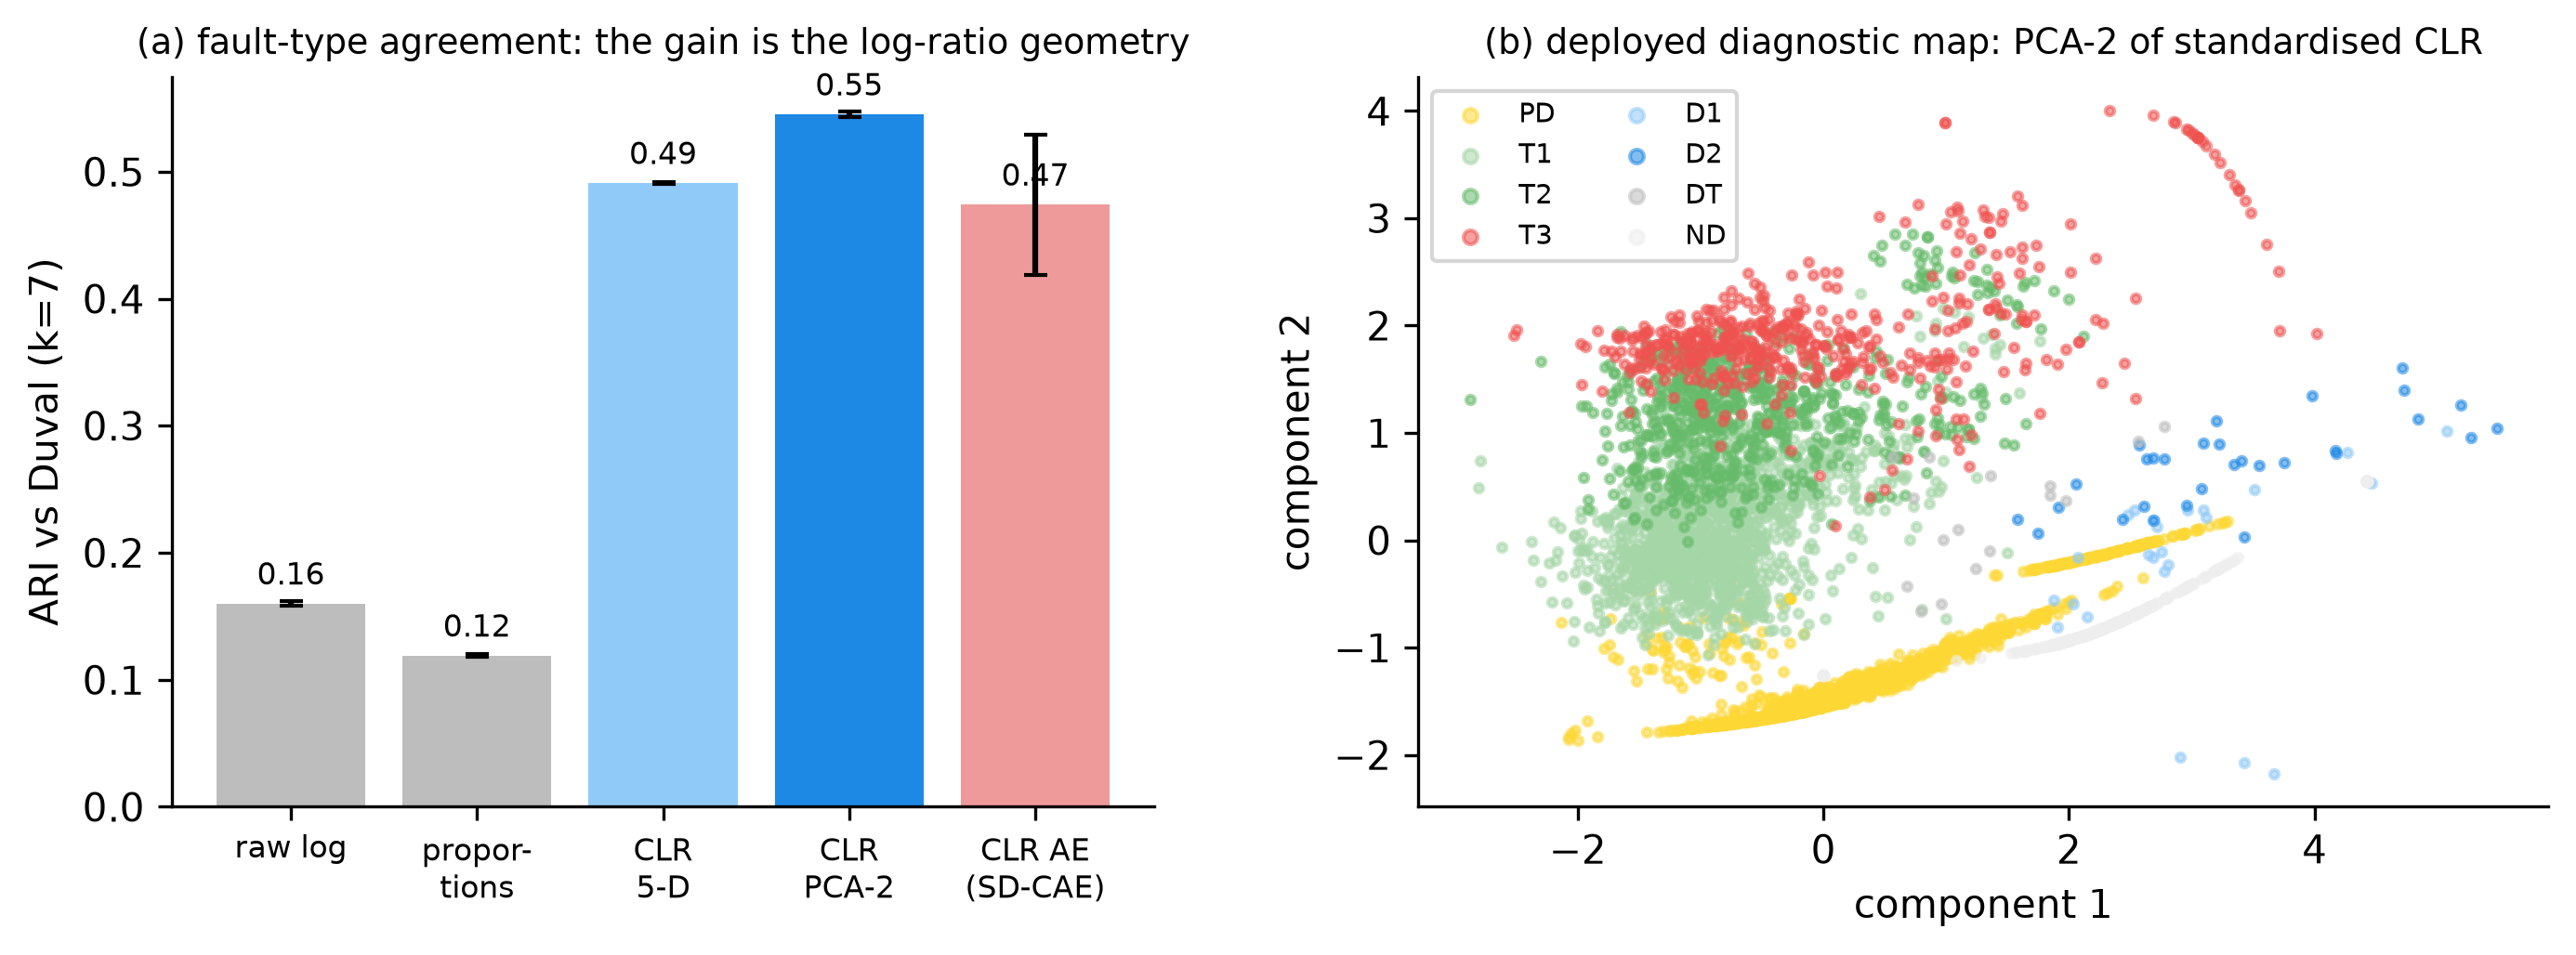
\includegraphics[width=0.9\textwidth]{representation_panel}
  \caption{Severity-disentangled compositional representation. (a) Fault-type agreement with
  Duval across representations (mean$\pm$std, five seeds): the gain comes from the CLR
  log-ratio geometry, and a linear PCA projection beats the SD-CAE autoencoder (negative
  ablation). (b) The deployed label-free diagnostic map---PCA-2 of the standardised
  CLR---coloured by Duval class; discharge (D1/D2), partial discharge, and thermal (T1--T3)
  regions separate.}
  \label{fig:repr}
\end{figure*}

\subsection{Label-free health/risk screening}
The risk index ranks the fleet with AUC~$0.74$ (unit-bootstrap $95\%$ CI $[0.68,0.80]$) against
\texttt{fault\_note}, versus $0.52$--$0.56$ for the conventional severity proxies---though a
trivial sample-count predictor reaches a statistically indistinguishable $0.76$ on this
confounded label (Fig.~\ref{fig:confound}a), so the comparison must be read against that floor
(Sec.~\ref{subsec:confound}). Its top decile carries a
$\sim$$2.4\times$ event rate and its top ten units a $\sim$$4.4\times$ rate; the event rate
falls from $\sim$27\% in the riskiest decile to $\sim$2\% in the safest, with the five riskiest
deciles above the fleet base rate (Fig.~\ref{fig:health}). A component ablation shows
the order of importance: severity ($0.64$) $\rightarrow$ $+$acetylene ($0.71$) $\rightarrow$
$+$temporal H2 rate ($0.73$) $\rightarrow$ $+$anomaly ($0.74$); acetylene-awareness is the
dominant lever, consistent with arcing being the most dangerous fault. Among anomaly detectors,
Isolation Forest ($0.60$) and autoencoder reconstruction ($0.58$) are weak but additive, whereas
Deep~SVDD collapses on this small tabular feature space (AUC $0.52$); a battery of nine standard
detectors yields no improvement over the deployed combination. The component set was chosen
during development with feedback from this same label, so the absolute AUC carries some design
optimism; the component ordering, not the third decimal, is the finding.

\begin{figure}[t]
  \centering
  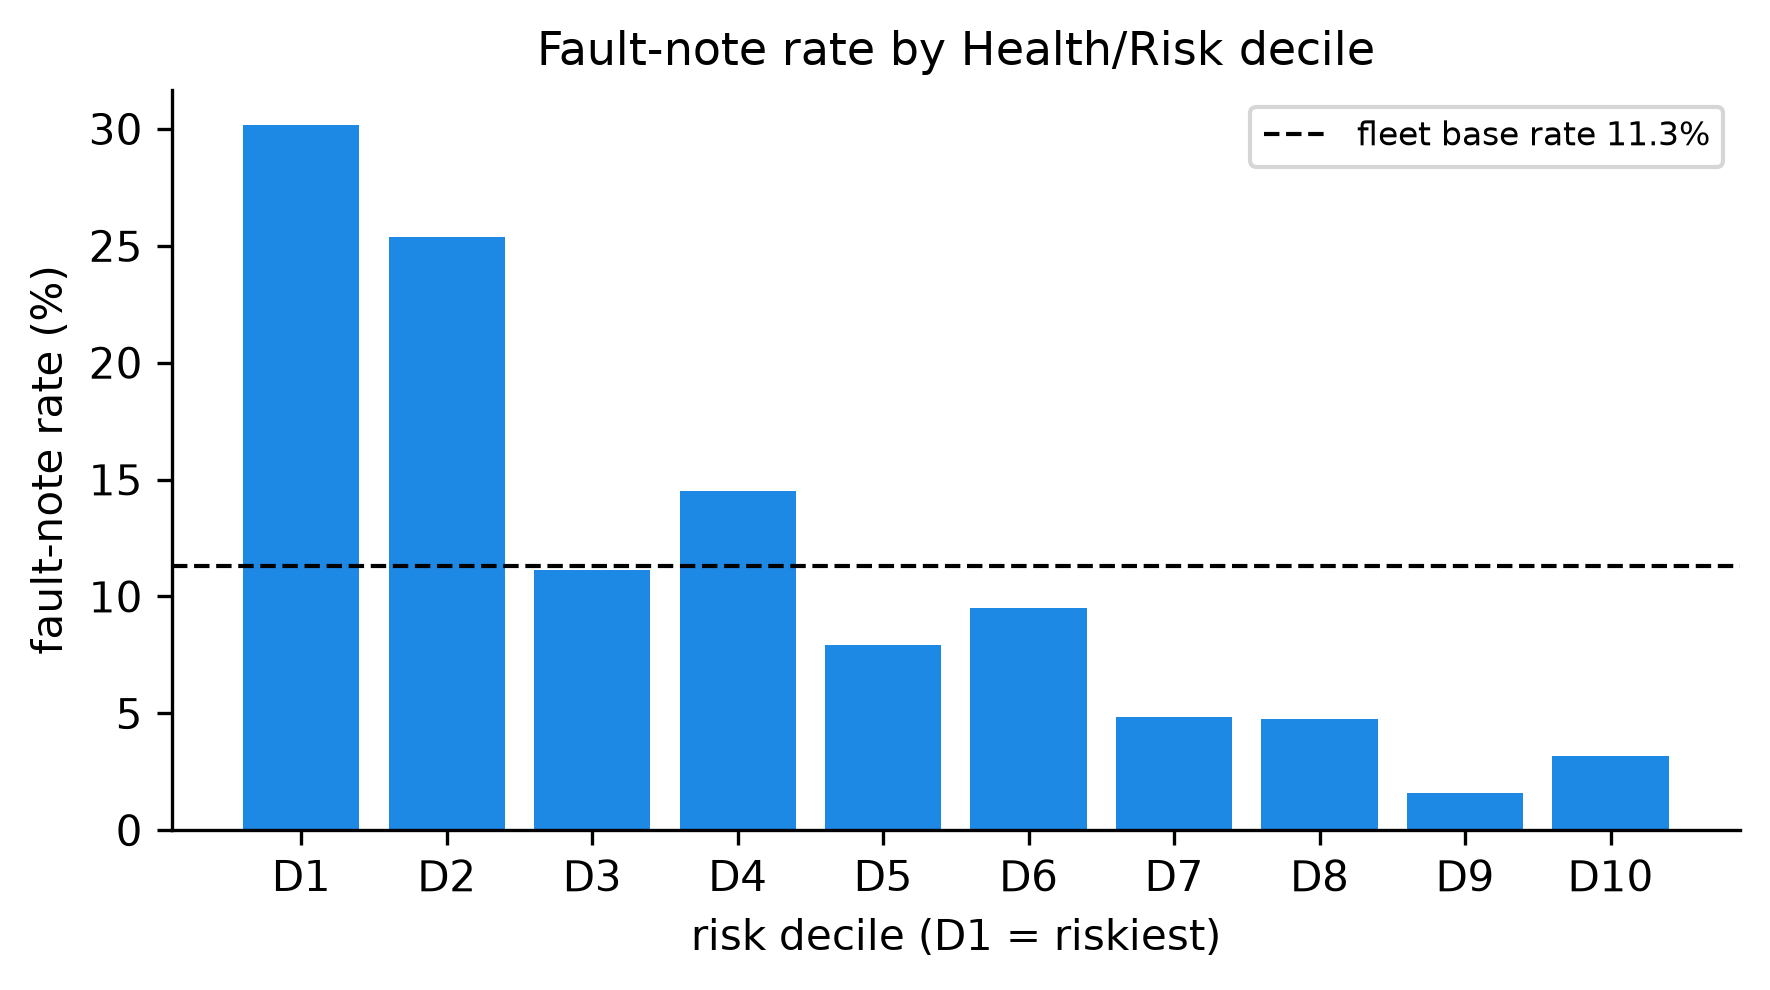
\includegraphics[width=0.92\columnwidth]{health_decile_note_rate}
  \caption{Field-event rate by health/risk decile (D1 = riskiest). The rate falls from
  $\sim$27\% (riskiest) to $\sim$2\% (safest); the five riskiest deciles exceed the fleet base
  rate (dashed).}
  \label{fig:health}
\end{figure}

\begin{figure*}[!t]
  \centering
  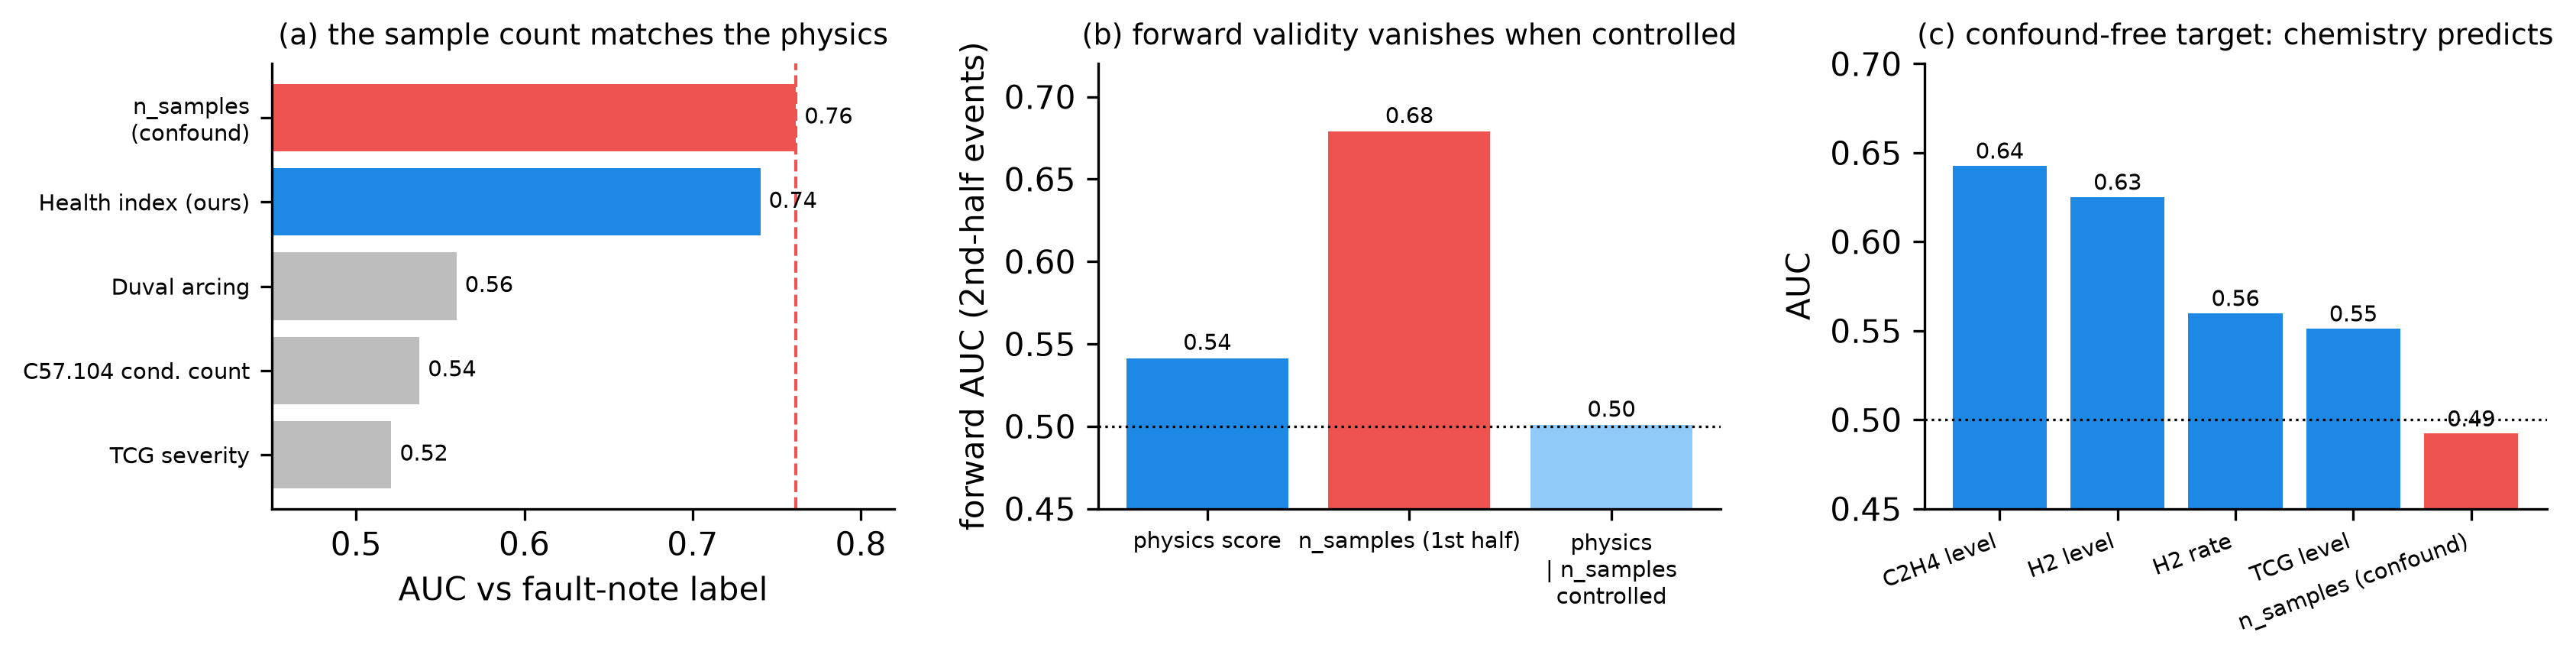
\includegraphics[width=0.93\textwidth]{confound_panel}
  \caption{The surveillance-bias analysis. (a) A trivial sample count matches the physics index
  against the field-note label and exceeds every conventional severity baseline (the confound
  floor). (b) Strict temporal hold-out: the score's forward validity vanishes once the
  sample-count confound is controlled, while the count alone forward-predicts. (c) Confound-free
  chemistry target (arcing onset): gas chemistry predicts, the sampling confound does not.}
  \label{fig:confound}
\end{figure*}

\subsection{The field-event label is surveillance-confounded}
\label{subsec:confound}
This is the paper's cautionary result. A trivial predictor---how many times a unit has been
sampled---scores AUC~$\mathbf{0.76}$ against \texttt{fault\_note}, statistically
indistinguishable from the physics index ($0.74$; paired-bootstrap difference CI
$[-0.10,+0.06]$, $p=0.58$) and far above the conventional baselines (Fig.~\ref{fig:confound}a).
The mechanism is operational: utilities re-sample units they are worried about, so the sample
count encodes attention rather than gas chemistry, and $69\%$ of the notes contain Thai text
largely missed by the English keyword label. In a joint logistic model the count adds signal
far beyond the physics (likelihood-ratio $p=9\times10^{-13}$) while the physics retains a
small significant increment ($p=0.003$): the label is dominated by, though not purely, operator
attention. Repairing the label with our Thai-note translation (six additional own-unit
electrical events) makes the count's advantage disappear entirely (AUC $0.734$ vs $0.735$),
indicating that part of its edge came from label incompleteness. The consequence is decisive
under a strict temporal hold-out: a label-free score built from each unit's first-half history
predicts second-half events at AUC $0.54$, the first-half sample count alone predicts them
better ($0.68$), and once the score is residualised on that count its forward AUC falls to
chance ($0.50$, Fig.~\ref{fig:confound}b). Because the first-half sample count is known
\emph{before} the second-half events, this is a prospective effect, not reverse causation. We
therefore do not claim genuine forward fault prediction from \texttt{fault\_note}; any AUC
against it must be read against the $0.76$ confound floor.

To evaluate without this confound we use a chemistry-defined target---the onset of arcing
(acetylene appearing within two years in a unit that has none), which is uncorrelated with the
sample count (correlation $-0.01$ with the target). Across 3{,}794 prediction points the
positives are rare and clustered: 45 positive points arising from only 17 onset units.
Accounting for this clustering with a unit-blocked bootstrap, ethylene and hydrogen forecast
onset at AUC $0.64$ ($95\%$ CI $[0.52,0.77]$) and $0.63$ ($[0.53,0.73]$)---both excluding
chance---while the sample count is uninformative ($0.49$, CI $[0.38,0.58]$,
Fig.~\ref{fig:confound}c); the result is robust across nine onset-threshold and horizon variants
(AUC $0.64$--$0.73$). Thermal activity (ethylene) and incipient hydrogen thus precede
arcing---a physically sensible, confound-free early signal, modest in effect size and with wide
intervals owing to the rarity of the event, but distinguishable from chance.

\section{Conclusion and Future Work}

We studied label-free condition monitoring of a real transformer fleet from Dissolved Gas
Analysis and reported three results. (1) A severity-disentangled compositional
representation---the centred log-ratio of the combustible-gas composition---recovers fault
\emph{type} by construction, raising agreement with the Duval classes from ARI $0.16$ to $0.55$
with a simple linear projection; the neural (SD-CAE) and adversarial-independence variants are
documented negatives. (2) The field-event notes commonly used to validate such models are, in
this fleet, confounded by surveillance bias: a trivial sample count matches the gas chemistry
(AUC $0.76$ vs $0.74$, difference not significant) and a label-free score built from these
features loses its apparent forward validity once that count is controlled. (3) A label-free
health/risk index nonetheless outranks conventional severity baselines, and on a confound-free,
chemistry-defined target the gas trajectory weakly forecasts the onset of arcing.

\textbf{Limitations.} The dataset has no ground-truth fault labels, so every result is measured
against a rule (Duval) or a weak, biased note label; the fault-type agreement is moderate; and
the findings come from a single fleet. The methods are deliberately simple---a linear projection
in the right geometry and small multilayer perceptrons---rather than a new architecture.

\textbf{Future work.} The highest-leverage improvement is a better target---completing the
domain validation of our Thai-note translation (which already recovers 15 missed event notes)
or obtaining real failure/maintenance records---after which the risk and prognostic claims can
be strengthened. We
also see promise in confound-free, chemistry-defined prognostic targets, in survival/remaining-
useful-life modelling of gassing trends, and, following recent surveys \cite{ramarao2026review},
in physics-informed and digital-twin extensions. More broadly, we recommend that DGA studies
which validate against operator-logged events report the sample-count confound floor, as a
trivial surveillance signal can otherwise be mistaken for diagnostic skill.


\bibliographystyle{IEEEtran}
\bibliography{references}

\end{document}
